\ylDisplay{Poldilõikur} % Ülesande nimi
{Mihkel Rähn} % Autor
{piirkonnavoor} % Voor
{2015} % Aasta
{G 7} % Ülesande nr.
{5} % Raskustase
{
% Teema: Staatika
\ifStatement
Leida, kui suurt jõudu avaldab poldilõikuri tera poldile (vt joonis), kui käepidemetele avaldatud jõud on $F = \SI{90}{N}$.
 \begin{center}
 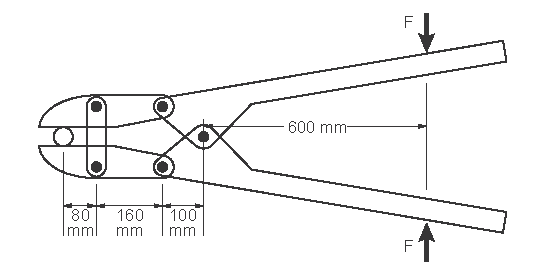
\includegraphics[width=0.7\textwidth]{2015-v2g-07-poldiloikur}
 \end{center}
\fi


\ifHint
Jõu ülekanne toimub kangi põhimõttel, kus summaarne jõumoment pöördtelje suhtes on võrdne nulliga. Vastavad jõumomentide tasakaalu saab kirja panna nii käepideme kui ka lõiketerade jaoks.
\fi


\ifSolution
Jõu ülekandmine toimub kangi põhimõttel, kus jõumoment pöördtelje suhtes summaarselt on võrdne nulliga. Käepideme korral
\[ \SI{600}{mm}\cdot\SI{90}{N}-\SI{100}{mm}\cdot F_k = 0 \quad\Rightarrow\quad F_k = \SI{540}{N}, \]
kus $F_k$ on käepidemetelt lõiketeradele mõjuv jõud. Analoogselt lõiketerade korral
\[ \SI{160}{mm}\cdot F_k - \SI{80}{mm}\cdot F_l = 0 \quad\Rightarrow\quad F_l = 2F_k, \]
kus $F_l$ on lõikuri poolt poldile avaldatud jõud.\\
Nendest võrranditest saame leida lõiketeradele mõjuva jõu $F_l$
\[ F_l = \SI{1080}{N}.\]
\fi


\ifEngStatement
% Problem name: Bolt cutter
Find how much force does the blade of the bolt cutter apply on the bolt (see figure) if the force applied on the handle is $F = \SI{90}{N}$.
\begin{center}
    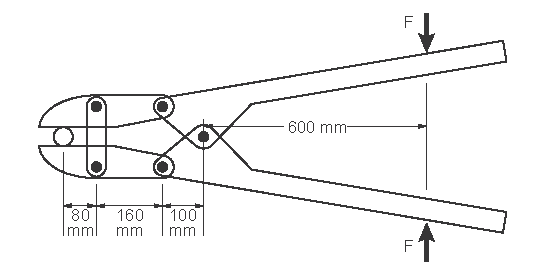
\includegraphics[width=0.7\textwidth]{2015-v2g-07-poldiloikur}
  \end{center}
\fi


\ifEngHint
You can apply the principle of moments for the force transmission where the total torque with respect to the axle of rotation is equal to zero. The corresponding torque balance can be written down for both the handle and the cutting blades.
\fi


\ifEngSolution
The force transmission is based on the principle of moments where the torque with respect to the turning axis by total is equal to zero. For the handle
\[ \SI{600}{mm}\cdot\SI{90}{N}-\SI{100}{mm}\cdot F_k = 0 \quad\Rightarrow\quad F_k = \SI{540}{N}, \]
where $F_k$ is the force applied to the blade by the handle. Similarly for the blades
\[ \SI{160}{mm}\cdot F_k - \SI{80}{mm}\cdot F_l = 0 \quad\Rightarrow\quad F_l = 2F_k, \]
where $F_l$ is the force applied to the bolt by the cutter.\\
From these equation we can find the force $F_l$ applied to the blades
\[ F_l = \SI{1080}{N}.\]
\fi
}